\documentclass[a4paper,12pt]{article}

\usepackage{latexsym}
\usepackage{amsfonts}
\usepackage{amsmath}
\usepackage{amsthm}
\usepackage{amssymb}
\usepackage{bbm}
\usepackage{graphicx}
\usepackage[normalem]{ulem}

\usepackage{hyperref}
\hypersetup{colorlinks=true,linkcolor=blue}

\usepackage{textcomp}
\usepackage{lmodern}
\usepackage[a4paper]{geometry}	
\usepackage[utf8]{inputenc}
\usepackage[T1]{fontenc}

\newcommand{\info}[1]{\texttt{#1}}

\begin{document}

\title{Lora's user manual}
\author{Laurent Claessens}
\maketitle

Lora is a backup program and a small Git remainder utility\footnote{Did you committed everything you modified today ?}.

\begin{center}
    {\bf Warning}
\end{center}
This is a free software\footnote{In the sense of the GPL : no warranty, etc.} manipulating your invaluable data. If you use it, I consider you as a consenting adult.

\tableofcontents

%+++++++++++++++++++++++++++++++++++++++++++++++++++++++++++++++++++++++++++++++++++++++++++++++++++++++++++++++++++++++++++ 
\section{Installation and compilation}
%+++++++++++++++++++++++++++++++++++++++++++++++++++++++++++++++++++++++++++++++++++++++++++++++++++++++++++++++++++++++++++

The first step is to download the whole on \href{ https://github.com/LaurentClaessens/lora  }{ github } with
\begin{center}
    \info{git clone https://github.com/LaurentClaessens/lora}
\end{center}


%--------------------------------------------------------------------------------------------------------------------------- 
\subsection{The manual way}
%---------------------------------------------------------------------------------------------------------------------------

\begin{enumerate}
    \item
        Create your \info{lora.cfg} looking at \info{example.cfg} for example and explanations.
    \item
        Modify the path of \info{BOOST\_THREAD\_LIB} in \info{makefile}.
    \item
        Test with
        \begin{center}
            \info{./tests.sh}
        \end{center}
        This should compile everything and launch a small testing program.
    \item
        Launch Lora with
        \begin{center}
            \info{./lora}
        \end{center}
\end{enumerate}

%--------------------------------------------------------------------------------------------------------------------------- 
\subsection{The graphical way}
%---------------------------------------------------------------------------------------------------------------------------

%///////////////////////////////////////////////////////////////////////////////////////////////////////////////////////////
\subsubsection{Compile the installation program}
%///////////////////////////////////////////////////////////////////////////////////////////////////////////////////////////

\begin{enumerate}
    \item
        Compile the installation program :
        \begin{center}
            \info{make installation}
        \end{center}
    \item
        Launch the installation program :
        \begin{center}
            \info{./installation}
        \end{center}
\end{enumerate}

%///////////////////////////////////////////////////////////////////////////////////////////////////////////////////////////
\subsubsection{The backup tab}
%///////////////////////////////////////////////////////////////////////////////////////////////////////////////////////////

Here it is :

\begin{center}
    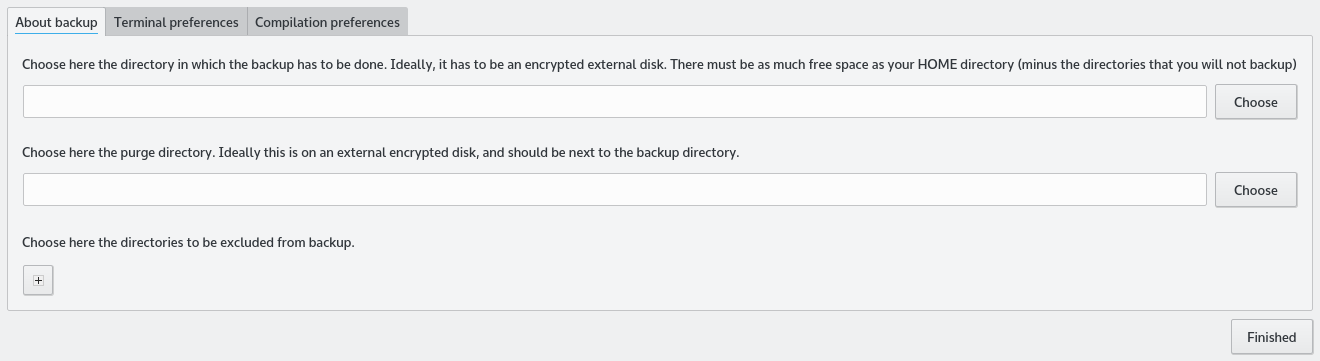
\includegraphics[width=\linewidth]{backup_tab.png}
\end{center}

\begin{enumerate}
    \item
        The backup directory (A) is the directory in which you want your \info{\$HOME} to be copied. Typically it will be something like
        \begin{center}
            \info{/mnt/backup\_partition/backup.lora}
        \end{center}
        where \info{/mnt/backup\_partition} is the mount point of an encrypted partition on an external drive.
    \item
        The purge directory (B) is the directory in which modified and removed files will be copied (from the backup directory) before to the respectively copied from the home to the backup and removed from the backup directory. The main user case is «I accidentally deleted a file, I perform the backup (thus the file is deleted from the backup) and \emph{then} I note that the file was removed.»  In this case, the removed file (in the version that was available in the backup) can be retrieved in the purge directory.

        Typically it will be something like
        \begin{center}
            \info{/mnt/backup\_partition/purge.lora}
        \end{center}

        Note that there are no automatic process removing the files from the purge directory. The size is then always increasing and you should remove very old subdirectory by hand.

        If you are using a program like Thunderbird, I let you know that it will \href{ http://xkcd.com/725/ }{ literally } produce \href{ https://fr.wikipedia.org/wiki/Gibioctet }{ gibis } of data in the purge directory each day.
    \item
        The excluded directories (C) are what they seem to be : they will be excluded from the backup. You can as example not backup the directory in which you save the \info{iso} files of your preferred Linux distribution. Press the 
\includegraphics{plus.png} button to add an excluded directory.
\end{enumerate}

%///////////////////////////////////////////////////////////////////////////////////////////////////////////////////////////
\subsubsection{The terminal tab}
%///////////////////////////////////////////////////////////////////////////////////////////////////////////////////////////

You can skip this if you don't use git. 

The ``Terminal tab'' allows you to determine what kind of terminal and editor you prefer\footnote{Serious people use \sout{gedit} vim or \sout{emacs}notepad. Under \sout{konsole}\,\sout{command.com}terminology.}.
Here is the tab :

\begin{center}
    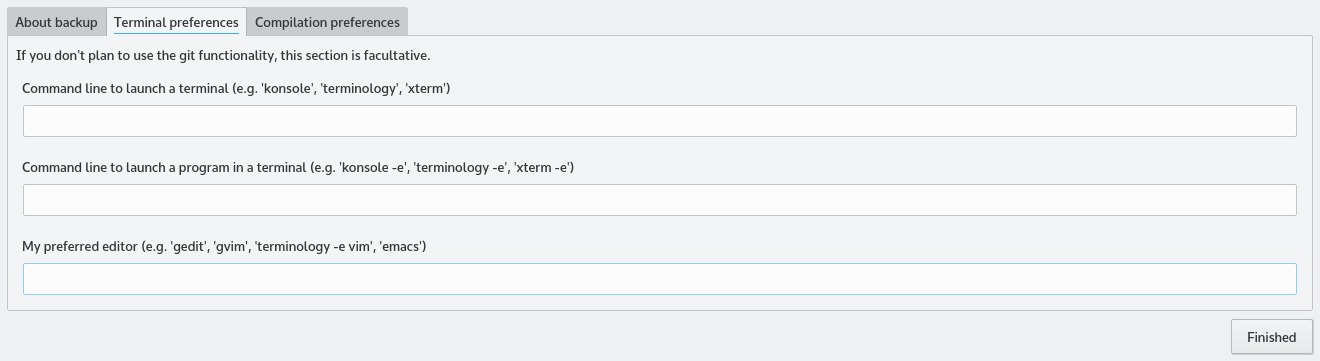
\includegraphics[width=\linewidth]{terminal_tab.png}
\end{center}
\begin{enumerate}
    \item
        The line (A) ask you the command line that launch your favorite terminal.
\end{enumerate}
<++>


\end{document}

    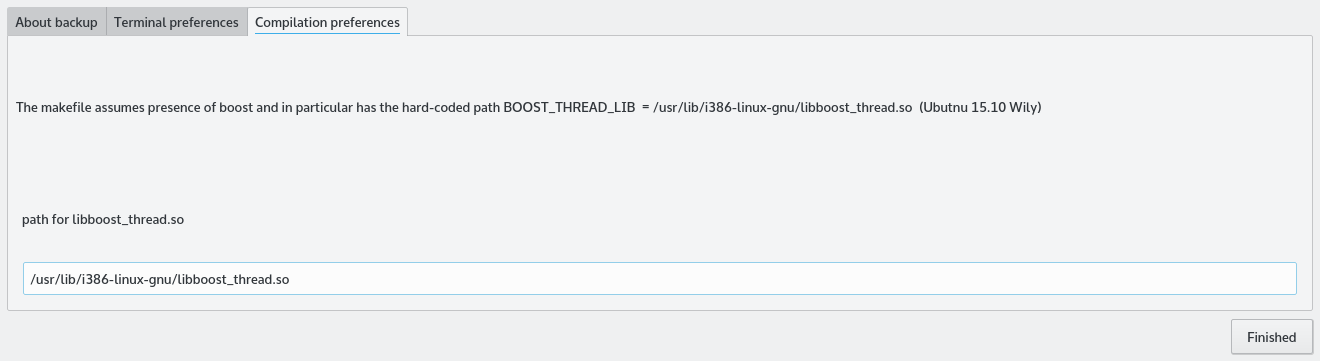
\includegraphics[width=\linewidth]{compilation_tab.png}



Compile the whole
    make all

NOTES
 
    You can bypass the installation if Boost is correctly located (see where the makefile assumes it is).  
Doing directly
        make all
works at my place (Ubuntu 15.10 Wily) 

    You can directly modify the 'lora.cfg' and 'makefile' file instead of using the installation program. 


DEFAULT USE

./lora 

will backup your $HOME directory using the backup and purge paths found in 'lora.cfg'

BACKUP A PART

./lora ~/foo

will backup the directory ~/foo in   <backup>/foo   where <backup> is the directory found in 'lora.cfg'. This contains the backup of $HOME.


USE AN OTHER CONFIG FILE

./lora --configuration=myconfig.cfg

will read the configuration file 'myconfig.cfg' instead of 'lora.cfg'


WHAT IS DOES -- BACKUP

The main feature is : the backup copy is only a copy. You can browse it with your favorite file browser and get a file back with a simple copy. You do not require a special software for getting back your data.

As an example, let us show how work the backup of $HOME=/home/daniel

We choose :
    backup directory : /mnt/baka/backup
    purge directory  : /mnt/baka/purge

Typically, /mnt/baka is the mount point of an encrypted external disk.


This software loops over the files and repertories of /home/daniel and creates a copy into
/mnt/baka/backup

At the end of the process, the directories /home/daniel and /mnt/baka/backup are the same (except for the excluded directories).

When making the backup of /home/daniel/bar/foo.txt,
* check if /mnt/baka/backup/bar/foo.txt
* if not, create it with a simple copy (but the last write time attribute is conserved)
* if /mnt/baka/backup/bar/foo.txt exists and is different
    - move to /mnt/backup/bakapurge.lora/<today date>/<hour>/modified/bar/foo.txt   (keeping the time attribute)
    - make the copy.

Thus the backup is incremental in the sense that the old version of a modified files is still available in a directory whose name is the date and the hour of the backup.



ATTENTION : There is no mechanism to suppress old file. Thus the size of directory /mnt/baka/purge is always increasing. This is by purpose : I prefer not have an automated way to suppress data.
    Consequence : some segmentation faults are triggered by "disk full". This is the user's responsibility to know what to suppress.

Trying to exclude a non-existing directory throws an error (when reading the configuration file). The reason roots in the following user case. Let suppose I don't want to
backup /home/daniel/videos/dvd (containing .VOB files) because it is very large and not really important. I add the line
exclude=/home/daniel/videos/dvd 
in the configuration file.
Now I change the directory name to /home/daniel/vidéos/dvd  (add an accent on "vidéo"). Then the backup process will copy the whole directory /home/daniel/vidéo and purge <purge>/videos. This is yet not really optimal, but copying the subdirectory /home/daniel/vidéos/dvd is REALLY what we don't want to do. 

When something strange happens, better to crash than silently manage the situation.


WHAT IT DOES -- PURGE

Lora loops over the directory /mnt/baka/backup and checks if these files correspond to files in /home/daniel.
When looking at /mnt/backa/backup/blah/stuff.tex

* check if /home/daniel/blah/stuff.tex exists
 - if yes, do nothing
 - if not, assume that this file was removed in the home and then move
/mnt/baka/backup/blah/stuff.tex ---> /mnt/baka/purge/<today date>/<hour>/removed/blah/stuff.tex


By the way, Lora has very bad performance against renaming an intere directory : in the first pass, it copy everything and in the second pass, it move the whole to the purge directory.

WHAT IT DOES -- GIT

Since Lora loops over the whole $HOME, it also take time to check for each directory if it is a git repository (has non trivial .git subdirectory) and if this repository
is clean.

A list of directories that are not clean git repository (untracked or modified files) is displayed. Clicking on one of them opens a dialog window that helps you to 
  - add files in .gitignore
  - add files
  - make a 'git commit -a'
  - see git diff
  - ...


